% LaTeX path to the root directory of the current project
\providecommand{\econtexRoot}{}
\renewcommand{\econtexRoot}{.}
% The \commands below are required to allow sharing of the same base code via Github between TeXLive on a local machine and ShareLaTeX.  This is an ugly solution to the requirement that custom LaTeX packages be accessible, and that ShareLaTeX seems to ignore symbolic links (even if they are relative links to valid locations)
\providecommand{\econtex}{\econtexRoot/LaTeX/texmf-local/tex/latex/econtex}
\providecommand{\econtexSetup}{\econtexRoot/LaTeX/texmf-local/tex/latex/econtexSetup}
\providecommand{\econtexShortcuts}{\econtexRoot/LaTeX/texmf-local/tex/latex/econtexShortcuts}
\providecommand{\econtexBibMake}{\econtexRoot/LaTeX/texmf-local/tex/latex/econtexBibMake}
\providecommand{\econtexBibStyle}{\econtexRoot/LaTeX/texmf-local/bibtex/bst/econtex}
\providecommand{\notes}{\econtexRoot/LaTeX/texmf-local/tex/latex/handout}
\providecommand{\handoutSetup}{\econtexRoot/LaTeX/texmf-local/tex/latex/handoutSetup}
\providecommand{\handoutShortcuts}{\econtexRoot/LaTeX/texmf-local/tex/latex/handoutShortcuts}
\providecommand{\handoutBibMake}{\econtexRoot/LaTeX/texmf-local/tex/latex/handoutBibMake}
\providecommand{\handoutBibStyle}{\econtexRoot/LaTeX/texmf-local/bibtex/bst/handout}
\providecommand{\economics}{economics}

\documentclass{beamer}
\usepackage{etoolbox}
\usepackage{comment}
\usepackage{graphicx}
%\usepackage{dtklogos}
\usepackage{dsfont}
\usepackage{amsmath,amssymb}
\usepackage{\econtexShortcuts}
\usepackage[english]{babel}
\usepackage[svgnames,hyperref]{}
\usepackage{empheq}
\usepackage[many]{tcolorbox}
\usepackage{remreset}
\usepackage{tikz} 
\usetikzlibrary{tikzmark,fit,shapes.geometric}
\usetikzlibrary{tikzmark,calc,arrows,shapes,decorations.pathreplacing}
\tikzset{every picture/.style={remember picture}}
\usepackage{cancel}
\usepackage{booktabs,natbib}
\setbeamercovered{invisible}

\usepackage{dcolumn}

\tcbset{highlight math style={enhanced,
		colframe=red!60!black,colback=yellow!50!white,arc=4pt,boxrule=1pt,
}}


\makeatletter
\@removefromreset{subsection}{section}
\patchcmd{\beamer@part}{\setcounter{subsection}{0}}{}{}
\makeatother
\setcounter{subsection}{1}
\setbeamercovered{transparent}
\setbeamertemplate{navigation symbols}{}%remove navigation symbols
\begin{comment}
\setbeamertemplate{footline}
{
	\hbox{\begin{beamercolorbox}[wd=1\paperwidth,ht=2.25ex,dp=1ex,right]{framenumber}%
			\usebeamerfont{framenumber}\insertframenumber{} \hspace*{2ex}
	\end{beamercolorbox}}%
	\vskip0pt%
}
\end{comment}


\mode<presentation>{}

\title[Modeling the Consumption Response to the CARES Act]{Modeling the Consumption Response\\ to the CARES Act}
\author[]{Christopher D. Carroll \and Edmund Crawley \and Jiri Slacalek \and Matthew N. White}
\date[04/21/2020]{April 21, 2020 \vspace{2cm} \\ \footnotesize Viewpoints and conclusions stated in this paper are the responsibility of the authors alone and do not necessarily reflect the viewpoints of the Federal Reserve Board or the ECB.}
\usetheme{Frankfurt}

\setbeamertemplate{navigation symbols}{}
\makeatletter
\setbeamertemplate{footline}
{%
	\hbox{\begin{beamercolorbox}[wd=1\paperwidth,ht=2.25ex,dp=1ex,right]{framenumber}%
		\usebeamerfont{framenumber}\insertframenumber{} \hspace*{2ex}
	\end{beamercolorbox}}%
	\vskip0pt%
	\pgfuseshading{beamer@barshade}%
	\ifbeamer@sb@subsection%
	\vskip-9.75ex%
	\else%
	\vskip-7ex%
	\fi%
	\begin{beamercolorbox}[ignorebg,ht=2.25ex,dp=3.75ex]{section in head/foot}
		\insertnavigation{\paperwidth}
	\end{beamercolorbox}%
	\ifbeamer@sb@subsection%
	\begin{beamercolorbox}[ignorebg,ht=2.125ex,dp=1.125ex,%
		leftskip=.3cm,rightskip=.3cm plus1fil]{subsection in head/foot}
		\usebeamerfont{subsection in head/foot}\insertsubsectionhead \insertframenumber{} \hspace*{2ex}
	\end{beamercolorbox}%
	\fi%
}%
\setbeamertemplate{headline}{%
}
\makeatother
\begin{document}
\setbeamertemplate{caption}{\raggedright\insertcaption\par}
\newcolumntype{d}[1]{D{.}{.}{#1}}
%circled draws a circle around a number
\newcommand*\circled[1]{\tikz[baseline=(char.base)]{
		\node[shape=circle,draw,inner sep=2pt] (char) {#1};}}

\begin{frame}[plain]
\titlepage
\end{frame}
\addtocounter{framenumber}{-1}
\section{Model}
\setbeamercovered{invisible}
\frame{
\frametitle{The CARES Act}
The CARES Act directly impacts household balance sheets:
\begin{itemize}
	\item \$1,200 to every adult (means tested)
	\item \$600 per week \textit{additional} unemployment benefits, for up to 13 weeks (\$7,800)
\end{itemize}
Compared to 10 years ago, we now have good models of how household consumption responds\\
\bigskip
Contribution of paper:
\begin{itemize}
	\item How is this time different?
	\item What does a carefully calibrated consumption model say?
\end{itemize}
}
\frame{
	\frametitle{What's Old - Baseline Model}
	We begin with a lifecycle model made up of high school dropouts, high school graduates and college graduates, matching:
	\begin{itemize}
		\item Their income profiles (trends and uncertainty)
		\item Liquid wealth	distribution (matched using patience heterogeneity)
	\end{itemize}
	This model has an annual Marginal Propensity to Consume (MPC) around 0.5\\
	\bigskip
	Matches \textit{both} micro and macro phenomena - e.g. \cite{psjmMPC2008}
}
\frame{
	\frametitle{What's New: (1) `Deep' Unemployment}
	We want to be able to experiment with different expectations (and realities) about the length of unemployment.\\
	Two types of unemployed:
	\begin{itemize}
		\item[1] `Normal' Unemployed: 2/3 probability of finding a job each quarter - expected unemployment duration 1.5 quarters
		\item[2] `Deep' Unemployed: 1/3 probability of returning to `normal' unemployed state each quarter - expected unemployment duration 4.5 quarters
	\end{itemize}
}
\frame{
	\frametitle{What's New: (2) `Lockdown' Consumption}
	Consumption during the lockdown is restricted: many forms of consumption are less desirable, or illegal
	\begin{itemize}
		\item We calibrate an 11 percent reduction in spending directly (from travel, restaurants, etc)
		\item We model this as a reduction in the marginal utility of consumption
	\end{itemize}
	Households prefer to defer some of their consumption into the future
}
\frame{
	\frametitle{Calibrating the Pandemic}
	We present two scenarios
	\begin{itemize}
		\item Short-Lived: The `lockdown' lasts two quarters on average, unemployment 15\% \\ One-third deep unemployment
		\item Long, Deep: The `lockdown' lasts four quarters on average, unemployment 22\%
		\\ Mostly deep unemployment
	\end{itemize}
	BUT these assumptions are highly contested and rapidly changing with data\\
	We invite you to make your own assumptions:\\
\hypertarget{links}{}
\begin{small}
	\parbox{\textwidth}{
		\begin{center}
			\begin{tabbing}
				\= \href{https://econ-ark.org/pandemicdashboard}{Interactive-Jupyter-Notebook} \= \textit{~~~~Allows user to modify some assumptions}                      \\
				\> \href{https://github.com/econ-ark/Pandemic}{github.com/econ-ark/Pandemic}   \> \textit{~~~~Full codebase} \\
			\end{tabbing}
		\end{center}
	}
\end{small}
}
\frame{
	\frametitle{Unemployment skewed young, unskilled and low income}
\begin{figure}
	\centering
	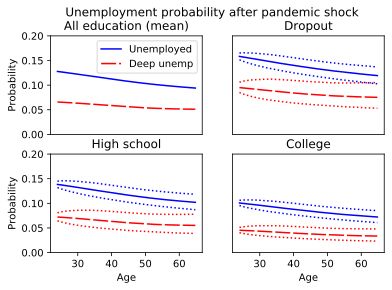
\includegraphics[width=0.9\textwidth]{\econtexRoot/Figures/UnempProbByDemogBasic}
\end{figure}
}
\frame{
	\frametitle{Aggregate Labor and Transfer Income}
	\begin{figure}
		\centering
		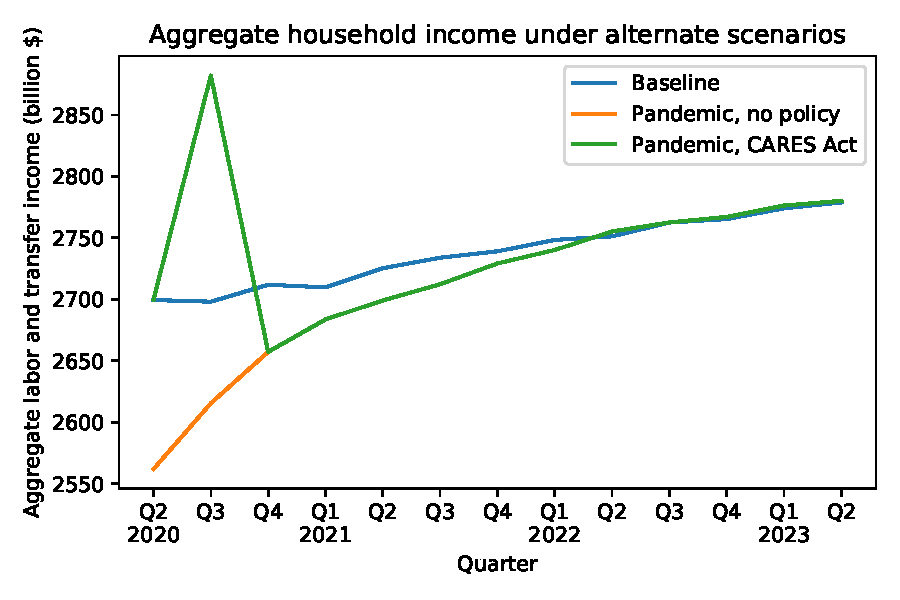
\includegraphics[width=0.9\textwidth]{\econtexRoot/Figures/AggLT}
	\end{figure}
	Assumption: Stimulus check delayed one quarter, 25 percent forward looking
}
\section{Results}
\frame{
	\frametitle{Aggregate Consumption Response}
	\begin{figure}
	\centering
	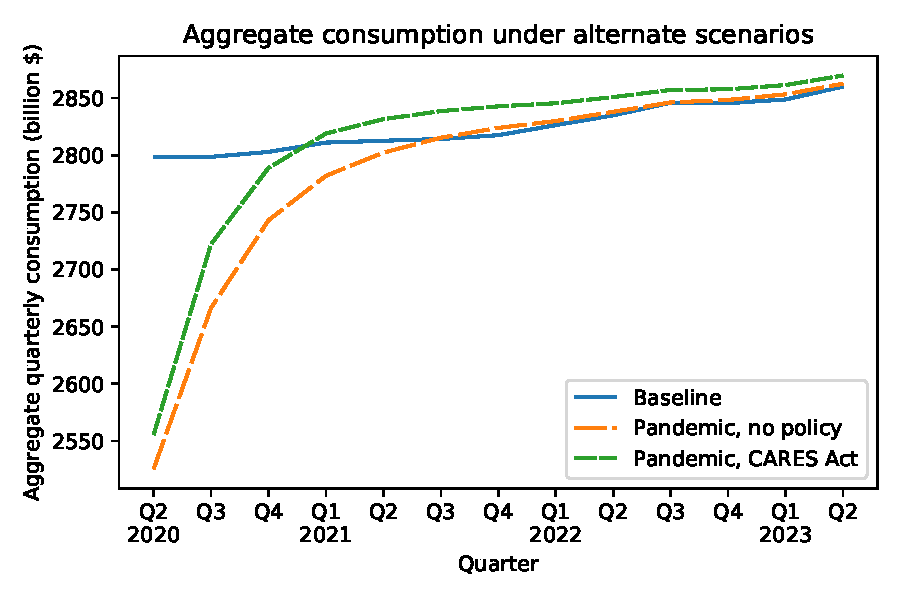
\includegraphics[width=0.9\textwidth]{\econtexRoot/Figures/AggConResp_examples}
\end{figure}
}
\frame{
	\frametitle{Consumption Response Decomposition}
	\begin{figure}
		\centering
		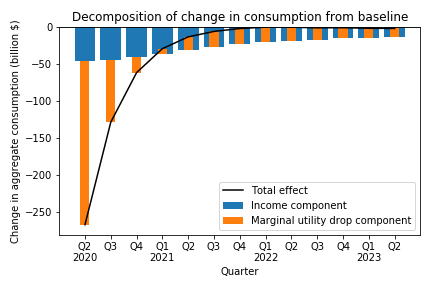
\includegraphics[width=0.9\textwidth]{\econtexRoot/Figures/Decomposition}
	\end{figure}
}
\frame{
	\frametitle{Consumption Response By Employment Type}
	\begin{tikzpicture}
	\node (img1) {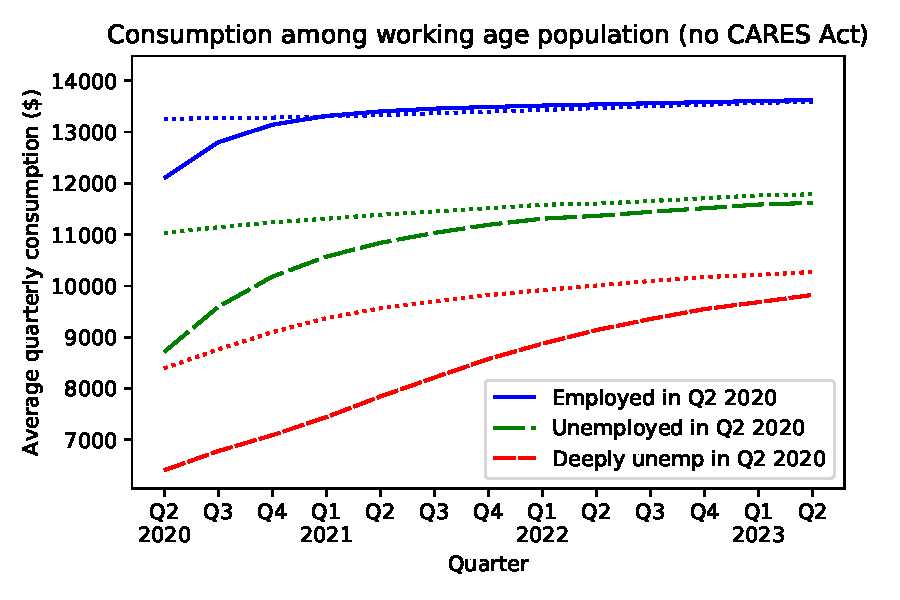
\includegraphics[width=0.9\textwidth,clip]{\econtexRoot/Figures/ConRespByEmpStateNoStim}};
	\pause
	\node (img2) {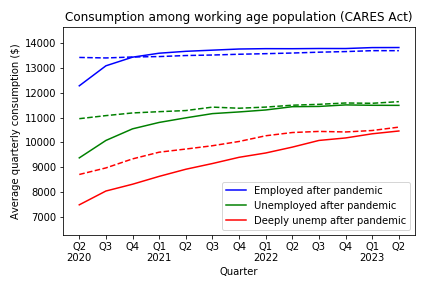
\includegraphics[width=0.9\textwidth,clip]{\econtexRoot/Figures/ConRespByEmpStateWStim}};
	\onslide<1->
	\end{tikzpicture}
}
\frame{
	\frametitle{Consumption Response By Employment Type}
	\begin{figure}
		\centering
		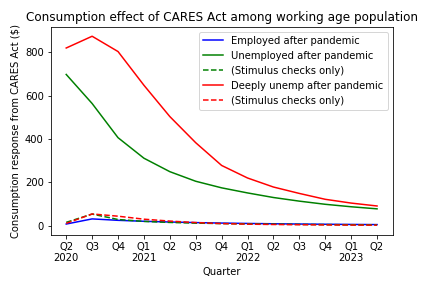
\includegraphics[width=0.9\textwidth]{\econtexRoot/Figures/ConDeltaByEmpState}
	\end{figure}
}
\frame{
	\frametitle{Is Targeting Useful In The Aggregate?}
	\begin{figure}
		\centering
		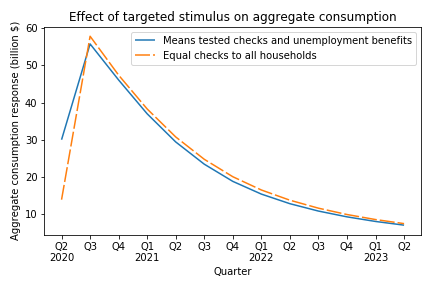
\includegraphics[width=0.7\textwidth]{\econtexRoot/Figures/EffectTargeting}
	\end{figure}
\begin{itemize}
	\item Deep unemployed have lower MPCs
	\item UE benefits are generous - average MPC lower than marginal
\end{itemize}
}
\frame{
	\frametitle{Deep, Long Pandemic: Income}
	\begin{figure}
		\centering
		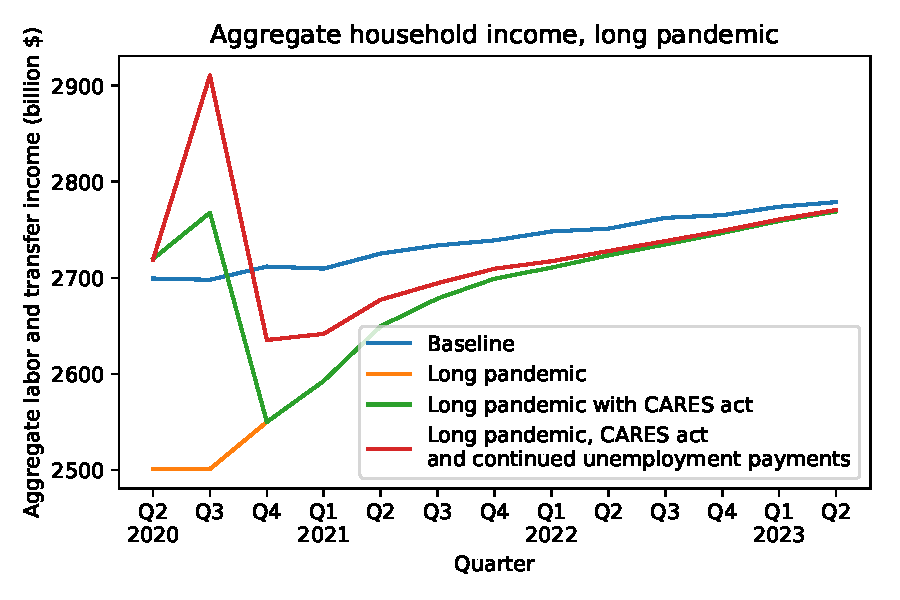
\includegraphics[width=0.9\textwidth]{\econtexRoot/Figures/AggLT_long_pandemic}
	\end{figure}
}
\frame{
	\frametitle{Deep, Long Pandemic: Consumption}
	\begin{figure}
		\centering
		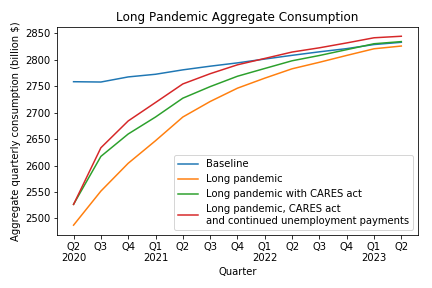
\includegraphics[width=0.9\textwidth]{\econtexRoot/Figures/DeepPandemic}
	\end{figure}
}
\frame{
	\frametitle{Conclusions}
	Short-lived lockdown: CARES Act looks sufficient for a swift recovery\\
	\bigskip
	Long, deep lockdown: Increased payments required to maintain demand\\
	\bigskip
	Check out the dashboard \url{https://econ-ark.org/pandemicdashboard}
}

\bibliographystyle{\econtexBibStyle}
\newsavebox\mytempbib
\savebox\mytempbib{\parbox{\textwidth}{\bibliography{\econtexRoot/LaTeX/ConsumptionResponse,\econtexRoot/LaTeX/ConsumptionResponse-Add}}}


\end{document}


